\section{Analyses}

Turmeric provides four modes of operation:

\begin{itemize}
    \item AC analysis
    \item Operating point analysis
    \item DC sweeping
    \item Transient analysis
\end{itemize}

\subsection{AC Analysis}

see AC.py, complex\_solve.py, LU.f90

\subsubsection{The Problem Statement}
AC analysis is a frequency domain phasor analysis. The simulation assumes no transient effects remain i.e the circuit has reached steady state conditions. Currently, \turmeric only supports linear circuit AC analysis.\\

Mathematically, the problem is as follows:
\begin{align*}
    &\left(\mathbf{D}\cdot j 2\pi f + \mathbf{M}\right)\cdot \colvec{x} + \colvec{Z}_{AC} = 0\label{eq:ac problem}\\\\
    &\mathbf{D}: \text{the dynamic matrix}\\
    &\mathbf{M}: \text{the reduced MNA matrix}\\
    &\colvec{Z}_{AC}: \text{the contribution of AC sources}\\
    &\colvec{x}: \text{the unknown node voltages and branch currents}\\
    &f: \text{the applied frequency}
\end{align*}

The circuit simulator evaluates the contribution of the dynamic matrix for a given frequency $\omega$. This calculation provides the effective impedance matrix. This impedance is summed with the $\mathbf{M}$ matrix to create a linear system of equations of the form:
\begin{align*}
    \mathbf{A}\colvec{x} - \colvec{b} = 0 
\end{align*}
\subsubsection{Dealing with Complex Valued Coefficients}
 It's not as simple as calling an LU algorithm to solve this problem as the system has complex valued coefficients. Python's numpy library has native support for complex values (as does FORTRAN's LAPACK), but it was important that we used no pre-built numerical programs. We opted to use the CR transformation to create $2\times$ equations with real-valued coefficients from $n$ equations with complex valued coefficients\cite{ercegovac_muller_2007}.\\
 
 \begin{figure}[!h]
     \centering
     \begin{align*}
     &x+jy \leftrightarrow
     \begin{pmatrix}
     x & -y \\
     y & x
     \end{pmatrix}
    \end{align*}
     \caption{$2\times 2$ skew symmetrix representation of a complex number}
     \label{fig:complex rep}
 \end{figure}
 
The \texttt{complex\_solve.solve} method operates as follows:
\begin{enumerate}
    \item[1.] Given a system of $n$ equations with complex valued coefficients, dynamically allocate empty zero matrices for the skew symmetric representation
    \item[2.] Map each complex coefficient (see \cref{fig:complex rep}) and position it inside the $2n \times 2n$ matrix (or $2n \times 1$ RHS)
    \item[3.] Solve the resulting system using an LU decomposition algorithm
    \item[4.] Convert the real valued solution to a complex valued array
\end{enumerate}

\subsubsection{Options for the user}
\turmeric provides logarithmic (default) and linear AC sweeping. The user specifies:
\begin{itemize}
    \item \texttt{nsteps} the number of simulation points
    \item \texttt{start} the start point: $x \overset{!}{>} 0$
    \item \texttt{stop} the stop point: $x \overset{!}{>} \text{start}$
    \item \texttt{sweep} LOG/LIN
\end{itemize}

An AC directive would look like this:

FILL IN DIRECTIVE HERE

\subsection{Operating Point Analysis}

see LU.f90, OP.py, schockley.py

An operating point analysis evaluates the node voltages and branch currents when there is no transient source. As a result, there are a number of simplifications the operating point analysis makes:

\begin{itemize}
    \item Capacitors are considered open circuits and inductors short circuits. As such they have no impact on the $\mathbf{M}$ matrix. Inductors behave as a short circuit \footnote{in the MNA equations, this is a 0 V voltage source}
    \item Furthermore, the system is static. There is no time derivative and as such contributions from the dynamic matrix are zero. \[\mathbf{D} = [0] \]
    \item Time-dependent voltage and current sources are open and short circuits respectively. Only DC contributions are considered \[ \colvec{Z}_{T}\left( t\right) = \colvec{0}\]
\end{itemize}

The operating point problem reduces to:

\begin{align*}
    &\mathbf{M}\cdot \colvec{x} + \colvec{N}\left(\colvec{x} \right) + \colvec{Z}_{DC} = 0 \label{eq:op problem}\\\\
    &\mathbf{M}: \text{the reduced MNA matrix}\\
    &\colvec{NL}\left(\colvec{x} \right): \text{the non-linear element contribution}\\
    &\colvec{Z}_{DC}: \text{the contribution of DC sources}\\
    &\colvec{x}: \text{the unknown node voltages and branch currents}
\end{align*}

\subsubsection{The Linear Case}

see LU.f90

If the circuit only consists of linear elements, the problem simplifies:
\begin{align*}
    &\colvec{NL}\left(\colvec{x} \right) \equiv \colvec{0}\\
    &\mathbf{M}\cdot\colvec{x} +\colvec{Z}_{DC} = 0
\end{align*}
This problem can be solved by means of a linear systems solver. \turmeric uses an LU decomposition method \cite{press1992numerical}. The solver was implemented in FORTRAN and compiled using \texttt{f2py}. In order to correctly interface with python, \texttt{f2py} requires explicit typing and some special directive comments to correctly track arguments with \texttt{inout} intent.\\

There are two functions in the \texttt{LU.f90} module:
\begin{itemize}
    \item \texttt{LUDCMP(A, N, INDX, D, CODE)} computes and returns a row-wise permutation of the $N \times N$ matrix A. INDX is a $N\times 1$ matrix which stores the row permutations. D, records an odd or even number of row changes. C is an error code indicating a singular matrix.
    \item \texttt{LUBKSB(A,N,INDX,B)} computes and returns the solution x for an $N\times N$ LU decomposition (A) using backward substitution
\end{itemize}

The most difficult simulation that \turmeric shows in this report is with a circuit whose MNA equations are approximately $20\times 20$. \Cref{fig:VS} gives an idea of the speed and efficiency of the FORTRAN LU solver in comparison with numpy's linear system solver. It isn't a fair test because \texttt{np.linalg.solve} implements a suite of solvers (ours is just LU) and has to test to see what is appropriate at runtime. It shows however, that at the lower matrix sizes, the algorithm is competitive.\\

\begin{figure}
    \centering
    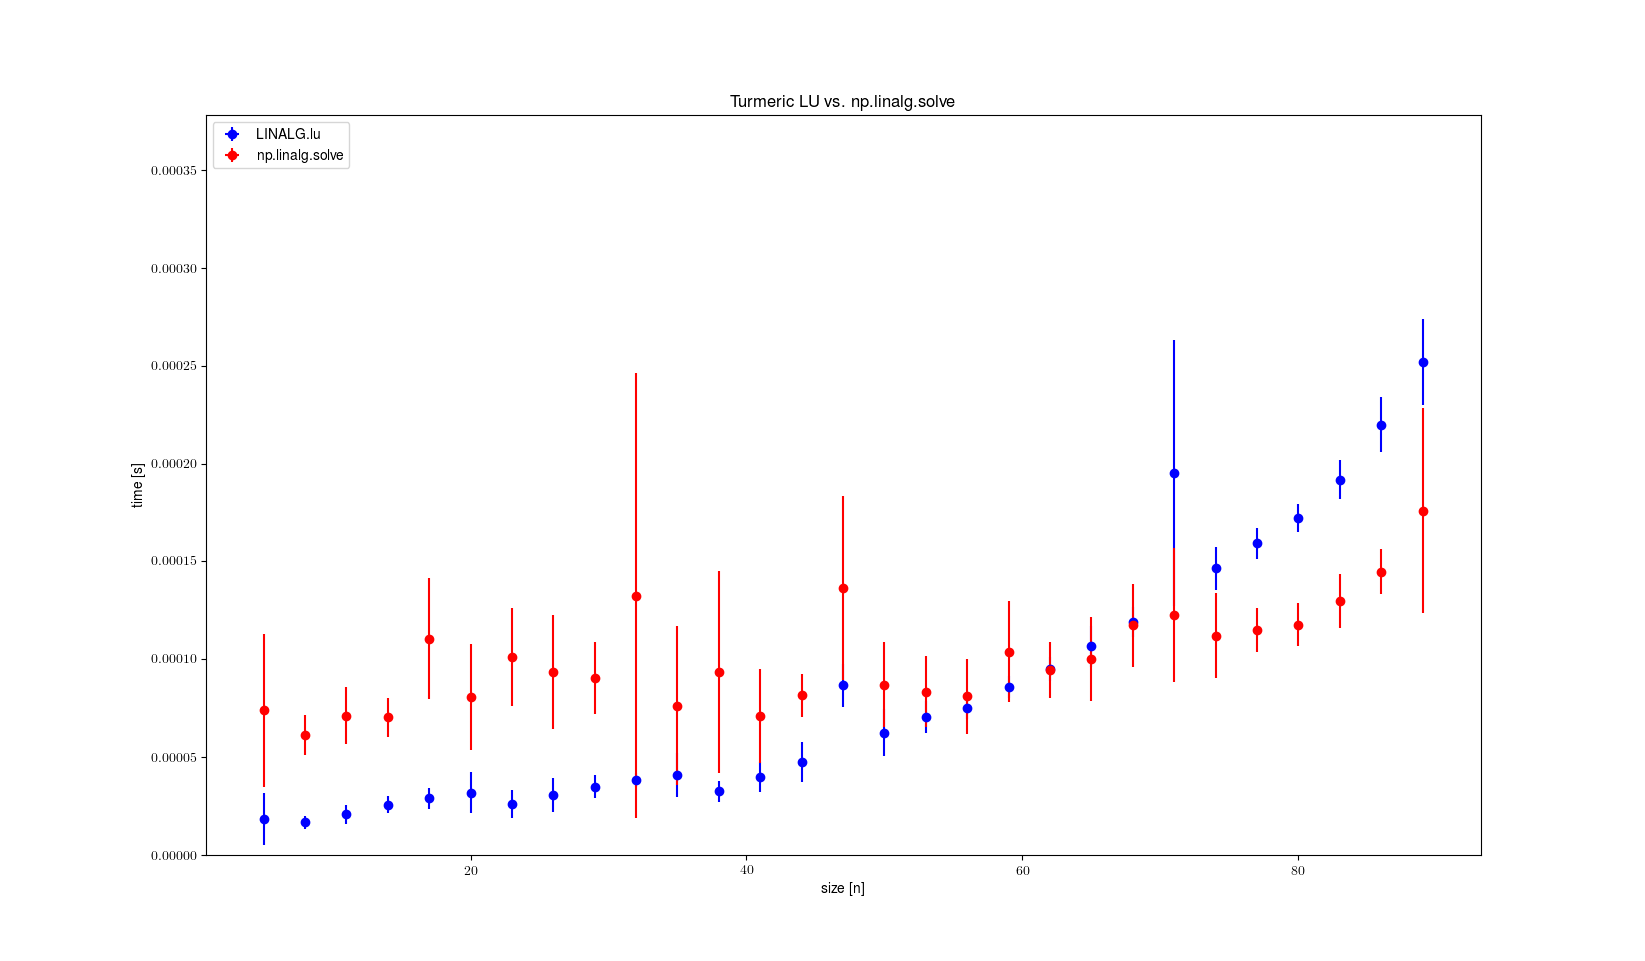
\includegraphics[width=\linewidth]{img/LUvnpsolve.png}
    \caption{Comparison of the \turmeric LU decomposition and numpy's linear systems solver. Each algorithm solved the same $N\times N$ linear system 5 times for a range of $N$. The average speed is given by a dot, and the standard deviation is marked with an error bar}
    \label{fig:VS}
\end{figure}

\subsubsection{The Non-Linear Case}

see OP.py (op\_analysis()), DC\_SUBRS.f90

If a circuit contains a non-linear element, there is a little more work to be done. The SPICE Book \cite{vladimirescu1994spice} details several methods of conditioning the MNA matrix to avoid singularities and to aid convergence. \\
\textbf{op\_analysis()}\\
Most texts recommend the use of a "$G_{min}$" matrix. This operates on the $M$ matrix by adding a small conductance ($G_{min}$) from each node to ground. A user can specify this conductance, but it defaults to $\SI{1d-12}{\siemens}$. The $G_{min}$ matrix ($\mathbf{G}$) is a zero matrix of the same size as $M$ is a zero matrix whose diagonal entries ($\mathbf{G}\left( i, i\right)$) up until the number of nodes (excluding the reference) are the $G_{min}$. The matrix is built in the FORTRAN module \texttt{DC\_SUBRS.f90}.\\

Providing an initial estimate for the operating point is \textit{recommended} if you are experiencing convergence issues. This estimate can be provided through the netlist. The $G_{min}$ matrix \texttt{op\_analysis()}\\

dc\_solve.py, solver.py

The MNA matrices are first passed to an intermediate function \texttt{dc\_solve()}


\texttt{solver.py} contains all of the solving methods implemented in \turmeric. At runtime, when the simulator reaches the \texttt{dc\_solve()} method, solver objects are initialised and stored in an ordered list. \turmeric currently implements:
\begin{itemize}
    \item \textbf{Standard Solving}: the MNA equations are not altered in any way. This method is used as an initial strategy
    \item \textbf{$G_{min}$ Stepping}: 
\end{itemize}


\begin{enumerate}
    \item[1.] The $M$ matrix is augmented by adding a small conductance ($G_{min}$) from each node to ground to aid convergence. A user can specify this conductance, but it defaults to $\SI{1d-12}{\siemens}$. The $G_{min}$ matrix ($\mathbf{G}$) is a zero matrix whose diagonal entries are the $G_{min}$. Mathematically, \[ \mathbf{G} = G_{min}\mathbf{I}\]
    
    THIS IS NOT THIS SIMPLE
    \item[2.] The system (after this operation) looks like this: \[ \left(M + G \right)\cdot \colvec{x} + \colvec{Z}_{DC} +  \colvec{N}\left(\colvec{x} \right) = 0\]
    This is an implicit equation in $\colvec{x}$ and can only be solved wth an iteration method. \turmeric employs a damped newton method with user modifiable maximum iteration and tolerance values. 
\end{enumerate}

\subsection{DC Sweep}
The DC sweep is a relatively simple simulation that builds upon the operating point simulation.\\

The user specifies a source label, and the simulator computes operating points for each value of the target voltage on a linear scale from the start to the stop value. \turmeric only supports linear source sweeping.

\subsection{Transient}
The transient simulation 


